\subsection{Trabajo de preparación}

\begin{figure}[ht]
    \centering
    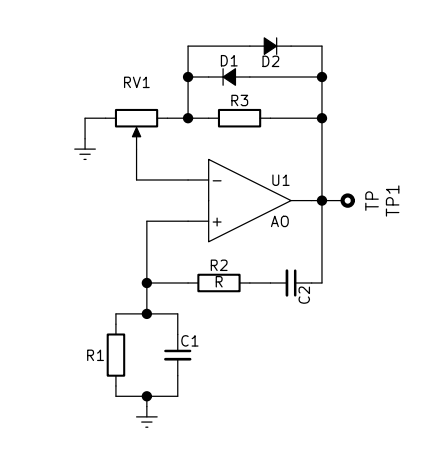
\includegraphics[width=0.5\textwidth]{oscilador-wien-control-amplitud.png}
    \caption{Oscilador de puente de Wien con control de amplitud}
    \label{fig:oscilador-puente-wien-control-de-amplitud}
\end{figure}

\paragraph{Para el circuito de la figura \ref{fig:oscilador-puente-wien-control-de-amplitud}, determinar la frecuencia de oscilación.\\}

Si se toma $R_1 = R_2 = R$ y $C_1 = C_2 = C$ La frecuencia de oscilación del circuito viene dada por la ecuación \ref{eq:frecuancia-corte-oscilador-wien}.

\paragraph{Diseñar (utilizando valores comerciales) el oscilador de la figura \ref{fig:oscilador-puente-wien-control-de-amplitud} con una frecuencia de oscilación de \\5.0 kHz.\\}

Partiendo de la ecuación \ref{eq:frecuancia-corte-oscilador-wien} primero fijamos el valor de los condensadores $C$ ya que se fabrican con mucho menos variedad de valores que las resistencias, En este caso se seleccionará

\begin{equation}
    \boxed{C = C_1 = C_2 = 10nF}
\end{equation}

Ahora hallamos el valor de la resistencia:

\begin{align}
    R &= \frac{1}{C \omega_o} \\
    R &= \frac{1}{10 nF \cdot 2\pi \cdot 5.0 kHz} \\
    R &= 3183\Omega
\end{align}

Un valor comercial cercano sería:

\begin{equation}
    \boxed{R = R_1 = R_2 = 3.3k\Omega}
\end{equation}

Ahora debemos cumplir con la condición $A = 3$, partiendo de la ecuación \ref{eq:ganancia-no-inversor} y tomando en cuenta que para este circuito:

\begin{align}
    R_f &= R_3 + xR_{v1} \\
    R_s &= (1-x) R_{v1}
\end{align}

tenemos

\begin{equation}
    A = 3 = 1 + \frac{R_3 + xR_{v1}}{(1-x)R_{v1}}
    \label{eq:ganancia-oscilador-lab}
\end{equation}

Si decimos que el potenciómetro tiene el valor

\begin{equation}
    \boxed{R_{v1} =  10k\Omega}
\end{equation}

y que $x = 0.5$, entonces tenemos

\begin{align*}
    3 &= 1 + \frac{R_3 + 5k\Omega}{5k\Omega} \\
    2 &= \frac{R_3 + 5k\Omega}{5k\Omega} \\
    10k\Omega &= R_3 + 5k\Omega \\
    R_3 &= (10 - 5)k \Omega \\
    R_3 &= 5 k\Omega
\end{align*}

usando un valor comercial

\begin{equation}
    \boxed{R_3 = 5.1 k\Omega}
\end{equation}

\paragraph{Determinar la amplitud de la señal de salida cuando está presente el control de amplitud\\}

Ahora, conectando los diodos al circuito en un principio no estarán funcionando, pero cuando el voltaje sea suficiente para polarizar los diodos estos entrarán en funcionamiento y toda la corriente pasará a traves de ellos en vez de por la resistencia $R_1$, por tanto la ecuación \ref{eq:ganancia-oscilador-lab} se vuelve

\begin{equation}
    A = 1 + \frac{x R_{v1}}{(1-x)R_{v1}}
\end{equation}

si decimos que $x=0$ 

\begin{align*}
    A &= 1 + \frac{0.5 R_{v1}}{0.5 R_{v1}} \\
    A &= 1 + 1 \\
    A &= 2
\end{align*}

Queremos encontrar la expresión de la tensión en la entrada negativa del amplificador $V_N$, para ello aplicamos un divisor de tensión desde $V_o$

\begin{align*}
    V_N &= \frac{(1-x)R_{v1}}{(1-x)R_{v1} + x R_{v1}}(V_o - V_{Don}) \\
    V_N &= \frac{(1-x)R_{v1}}{(1-x +x)R_{v1}}(V_o - V_{Don})\\
    V_N &= \frac{(1-x)R_{v1}}{R_{v1}}(V_o - V_{Don}) \\
    V_N &= (1-x)(V_o - V_{Don}) \\
    V_N &= (1-x)V_o - (1-x)V_{Don} 
\end{align*}

Recordando que 

\begin{equation}
    \frac{V_o}{V_N} = 3
\end{equation}

\begin{align*}
    \frac{V_o}{3} &= (1-x)V_o - (1-x)V_{Don} 
\end{align*}

despejamos $V_o$

\begin{equation}
    V_o = \frac{(1-x)V_{Don}}{1-x - \frac{1}{3}}
\end{equation}

\paragraph{}

\FloatBarrier
\subsection{Simulaciones}

\begin{ilustracion}[hb]
    \centering
    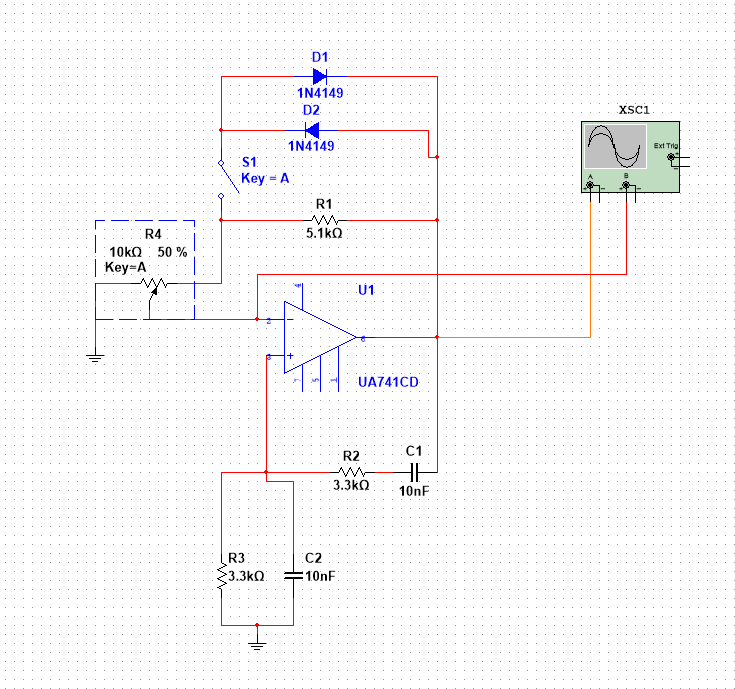
\includegraphics[width=0.5\textwidth]{simulaciones/sim-circuito.png}
    \caption{Circuito oscilador en el simulador}
    \label{ilus:simulacion-circuito}
\end{ilustracion}

El la ilustración \ref{ilus:simulacion-circuito} se muestra el montaje del circuito oscilador en el programa Multisim.

\begin{ilustracion}[hb]
    \centering
    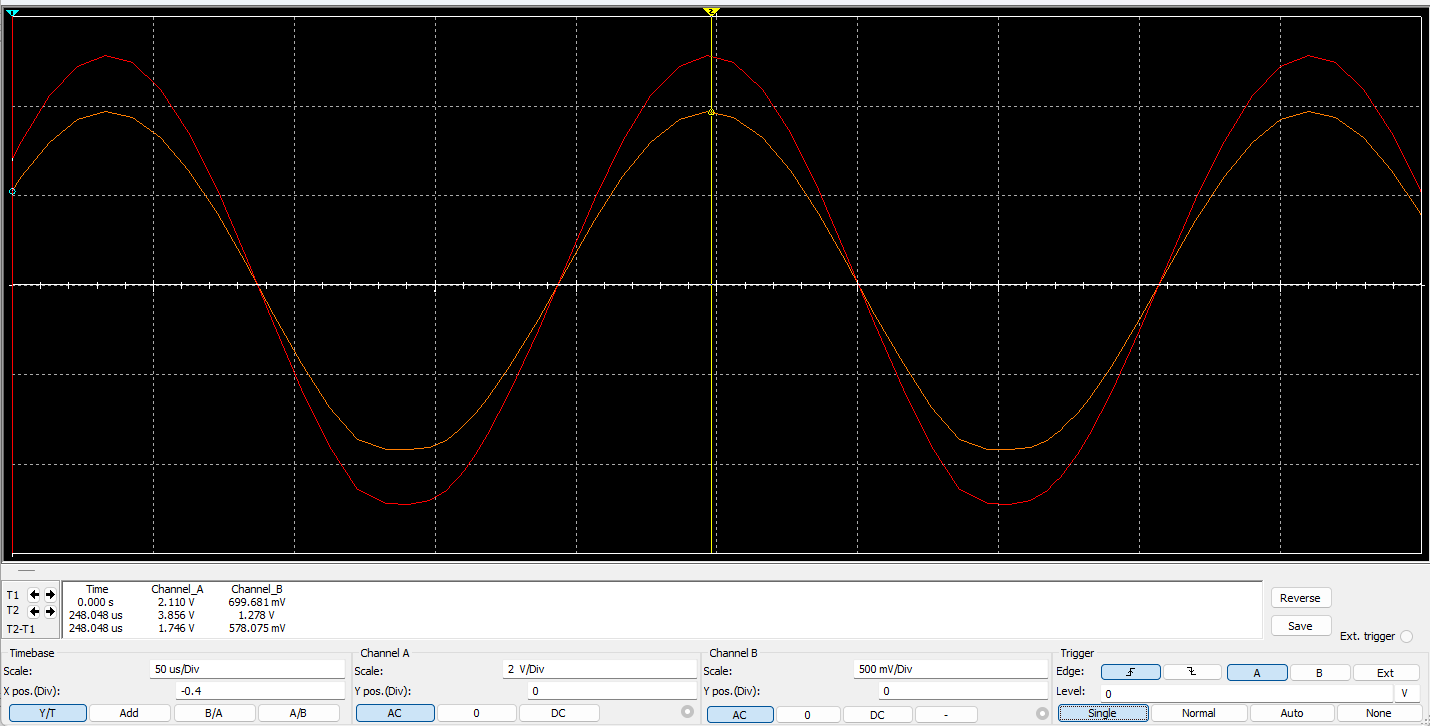
\includegraphics[width=0.5\textwidth]{simulaciones/forma-onda-sin-diodos.png}
    \caption{Forma de onda circuito oscilador sin control de amplitud}
    \label{ilus:simulacion-onda-sin-control-amplitud}
\end{ilustracion}

La ilustración \ref{ilus:simulacion-onda-sin-control-amplitud} muestra la forma de onda de la señal de salida del oscilador sin control de amplitud y con $x=0.5$. Podemos observar que la ganancia es 3.02 y la frecuencia de la señal es 4.76 kHz.

\begin{ilustracion}[hb]
    \centering
    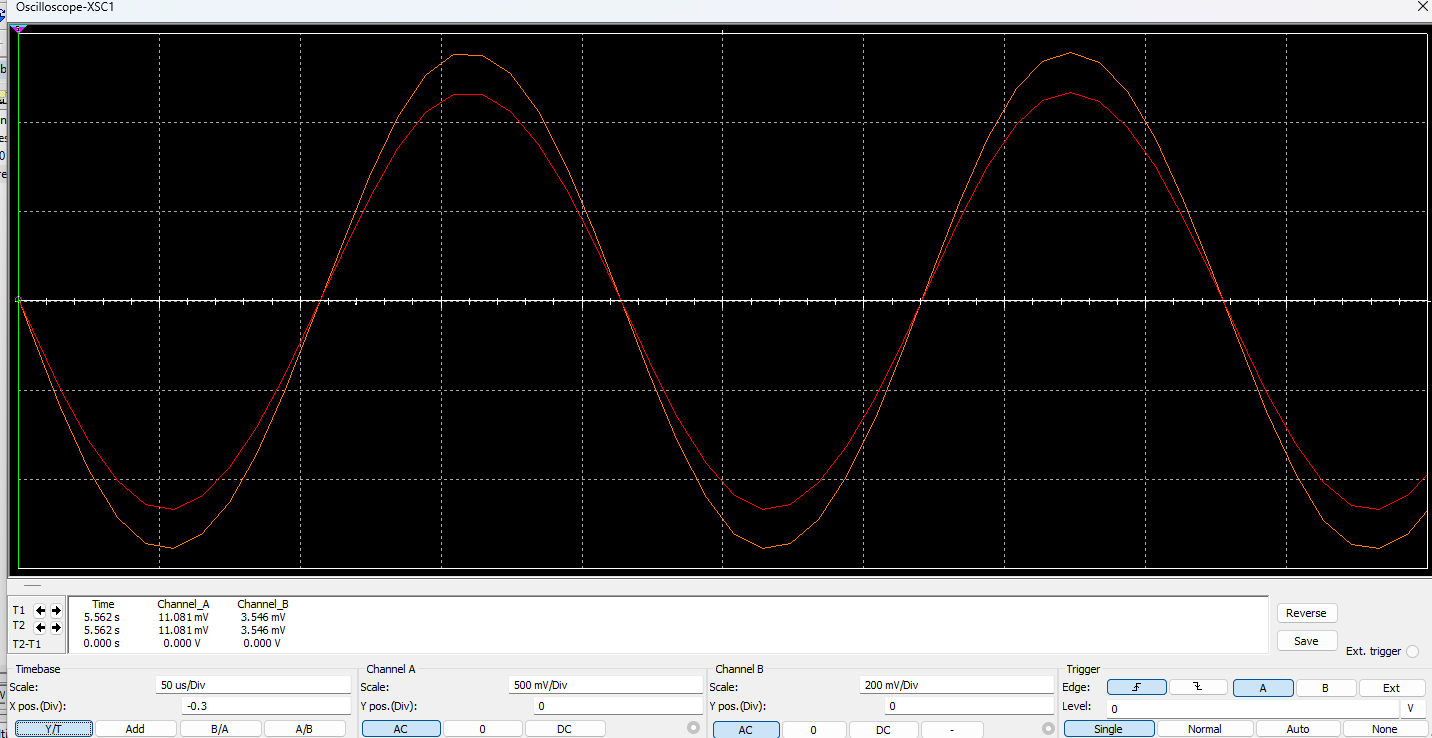
\includegraphics[width=0.5\textwidth]{simulaciones/forma-onda-con-diodos.png}
    \caption{Forma de onda circuito oscilador con control de amplitud}
    \label{ilus:simulacion-onda-con-control-amplitud}
\end{ilustracion}

La ilustración \ref{ilus:simulacion-onda-con-control-amplitud} muestra la forma de la onda del circuito oscilador con control de amplitud cuando $x = 0.5$, podemos observar que la ganancia es 2.98 y la frecuencia es 4.76 kHz.


\begin{ilustracion}[hb]
    \centering
    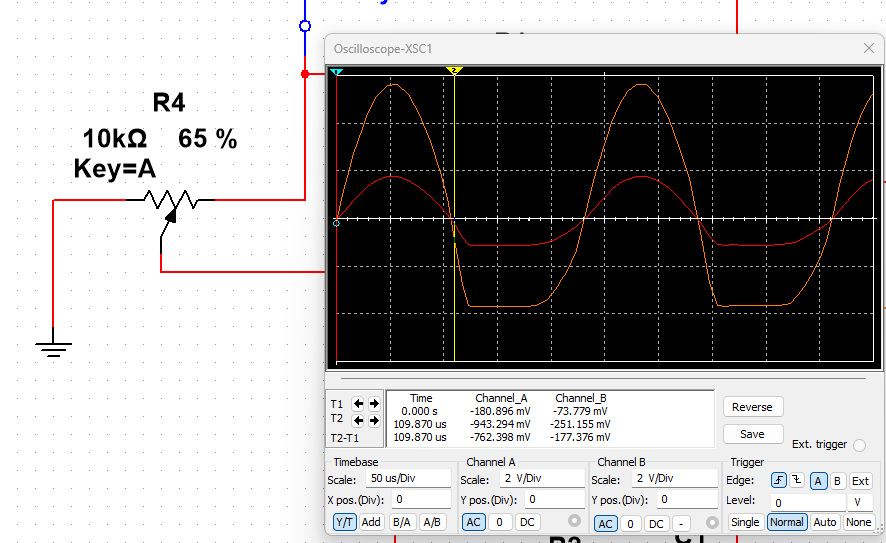
\includegraphics[width=0.5\textwidth]{simulaciones/forma-onda-con-diodos-x-65.png}
    \caption{Forma de onda circuito oscilador con control de amplitud cuando x=0.65}
    \label{ilus:simulacion-onda-con-control-amplitud-65}
\end{ilustracion}

En la ilustración \ref{ilus:simulacion-onda-con-control-amplitud-65} se observa que la onda se empieza a saturar y que la frecuencia se empieza a alejar de la condición $f=5kHz$.

\begin{ilustracion}[hb]
    \centering
    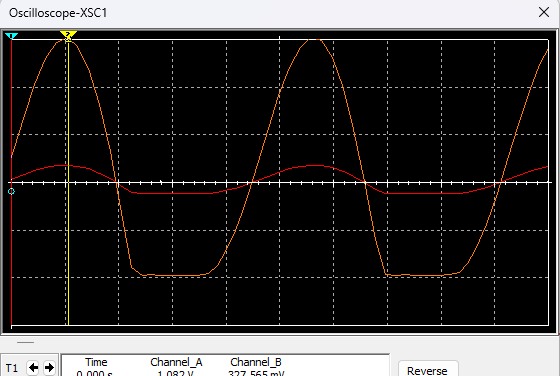
\includegraphics[width=0.5\textwidth]{simulaciones/forma-onda-sin-diodos-x-55.png}
    \caption{Forma de onda circuito oscilador sin control de amplitud cuando x=0.55}
    \label{ilus:simulacion-onda-sin-control-amplitud-55}
\end{ilustracion}

En la ilustración \ref{ilus:simulacion-onda-sin-control-amplitud-55} podemos ver que la onda se atenúa y la frecuencia se hace 4.34 kHz, alejándose de la frecuencia deseada de 5kHz.

De las simulaciones podemos observar que para el circuito sin control de amplitud el rango efectivo del potenciómetro es muy reducido, x debe ser muy cercano a 0.5, mientras que para el circuito con control de amplitud el rango de x aumenta hasta casi $x = \pm 0.65$. En la práctica de laboratorio se desea comprobar si el rango efectivo de x aumenta cuando se implementa el control de amplitud.